\chapter{Statistics}

\section{Hyphotesis Testing}

Sea $X_1, \dots X_n$ una muestra aleatoria de una distribución con densidad $f(x|\theta)$ con el parámetro $\theta \in \Omega$ (espacio de parámetros). Consideremos $\Omega_0$ y $\Omega_1$ disjuntos tales que $\Omega_0 \cup \Omega_1 = \Omega$. Un test de hipótesis se configura de la siguiente forma 

\begin{equation*}
\begin{aligned}
    H_0: \theta \in \Omega_0 \\ 
    H_A: \theta \in \Omega_1
\end{aligned}
\end{equation*}

Donde $H_0$ es la hipótesis nula y $H_A$ la hipótesis alternativa. El objetivo de un test de hipótesis es determinar si bajo $H_0$ es estadísticamente posible muestrear $X_1 , \dots, X_n$, o bien, se debiera considerar $H_1$.

\subsection{Mean of Normal Distribution - Known Variance}

Consideremos $X_1 , \dots X_n \sim \mathcal{N}(\mu, \sigma^2)$ con $\sigma^2$ un parámetro conocido. El test que planteamos es 
\begin{equation*}
\begin{aligned}
    H_0: \mu = \mu_0 \\ 
    H_A: \mu \neq \mu_0
\end{aligned}
\end{equation*}

Bajo la hipótesis $H_0$, suponemos que $X_1, \dots X_n \sim \mathcal{N}(\mu_0, \sigma^2)$. Por teorema del límite central, recordemos que 

$$ 
Z_n = \frac{\overline{X} - \mu_0}{\sigma / \sqrt{n}} \sim \mathcal{N}(0,1)
$$

Definimos el \textbf{p-valor} según
$$
\text{p}_{\text{value}} = P(|Z_n| \geq |z| \hspace{0.1cm} |\hspace{0.1cm} H_0) 
$$

Con $z$ el valor empírico obtenido de una muestra. Rechazamos la hipótesis nula cuando el p-valor es menor o igual que un nivel de significancia $\alpha$ (usualmente 1\%, 5\%, 10\%).

\begin{figure}[H]
    \center
    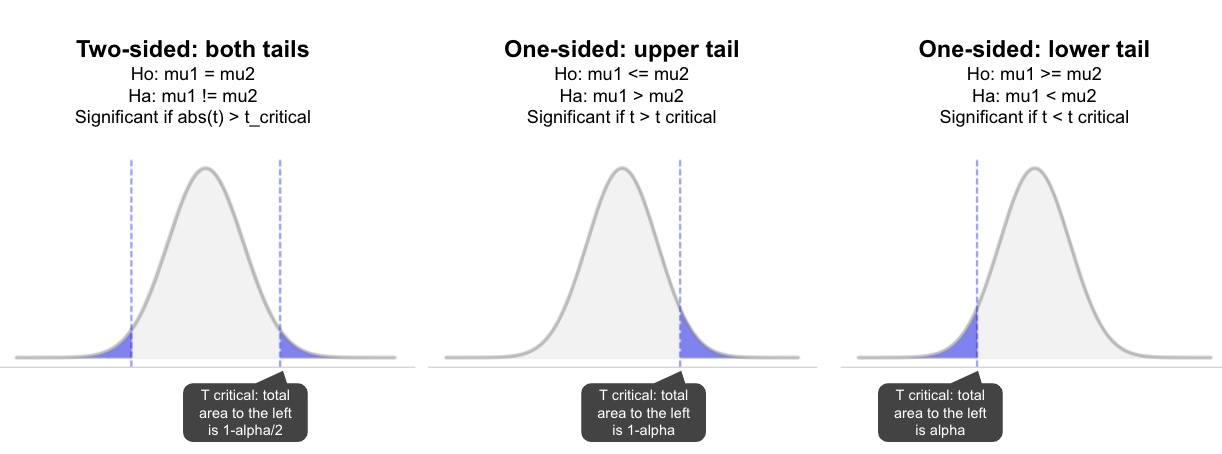
\includegraphics[scale=0.65]{notebooks/STATS/img/two_sided_test.png}
    \caption{One and Two Sided Test Diagram}
\end{figure}


Cuando rechazamos la hipótesis nula de manera errónea, le llamamos \textbf{error tipo I}, cuando no rechazamos la hipótesis nula siendo esta falsa, le llamamos \textbf{error tipo II}.

\begin{figure}[H]
    \center
    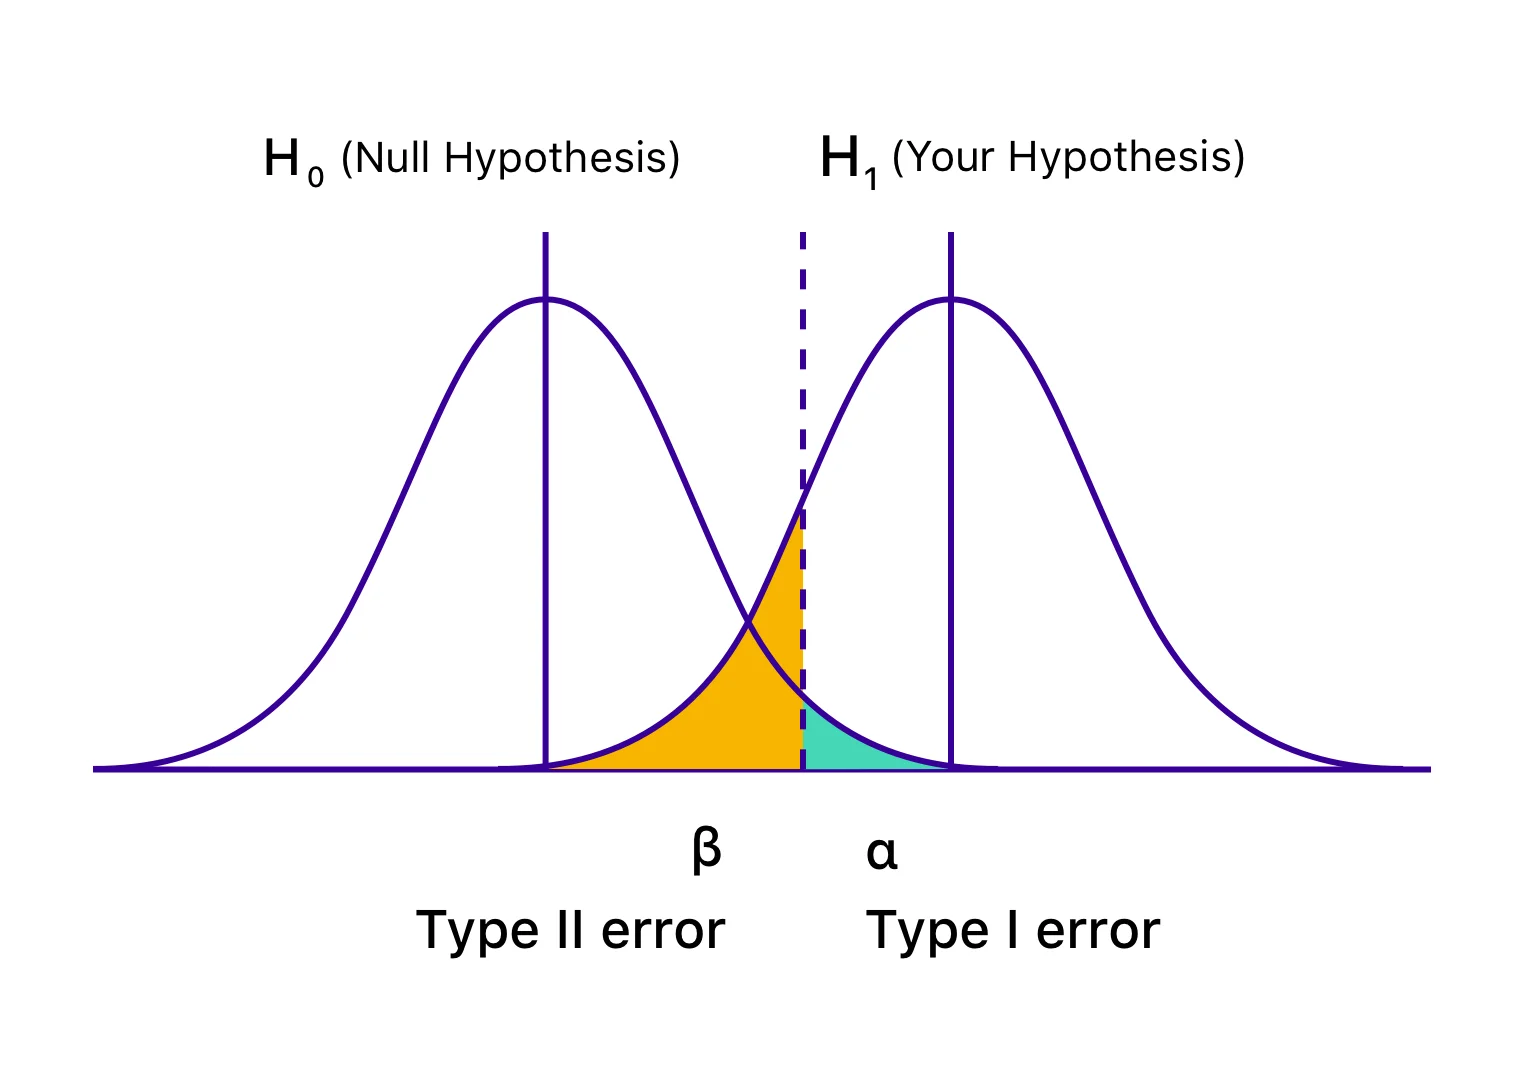
\includegraphics[scale=0.2]{notebooks/STATS/img/type_of_errors.png}
    \caption{Types of Errors Diagram}
\end{figure}

\subsection{Mean of Normal Distribution - Unknown Variance}

Cuando no conocemos la varianza de la distribución, el estadístico $Z_n$ se puede escribir según 
$$ 
t = \frac{\overline{X} - \mu_0}{s / \sqrt{n}}
$$
Con $s$ la desviación estándar de la muestra $X_1 , \dots, X_n$. En este caso, $t \sim T_{\text{student}}(n-1)$ una distribución t-student con $n-1$ grados de libertad. 

\subsection{Proportion Test}

Sea $X_1 \dots X_n \sim \text{Bernoulli}(p)$, definimos el test 

\begin{equation*}
\begin{aligned}
    H_0: p \geq p_0 \\ 
    H_A: p < p_0
\end{aligned}
\end{equation*}

Nuevamente, bajo la hipótesis nula $p = p_0$ por TCL para $n$ grande
$$ 
\overline{X} = \hat{p} \sim \mathcal{N} \left ( p_0 , \frac{p_0(1-p_0)}{n} \right )
$$
Es decir, el estadístico queda definido por $Z = \frac{\hat{p} - p_0}{\frac{\sqrt{p_0(1-p_0)}}{n}}$. 

\section{AB Testing}

Un AB Testing es un procedimiento que involucra dividir la población en un grupo de control y un grupo de tratamiento para testear 2 versiones de una única variable. El objetivo es determinar si la estrategia $A$ es más efectiva que una estrategia $B$ para alguna medida de interés.

\subsection{Experiment Design}

Es importante \textbf{aislar cualquier fuente de bias} que pueda estar presente entre el grupo de control y el grupo de tratamiento (cuando esto no es posible, le llamamos \textit{Quasi-Experimental} y se debe trabajar con \textit{Causal Inference}). 

Existen distintas formas de realizar esta separación, entre las que se incluyen: 

\begin{enumerate}
    \item \textbf{Randomized}: Cada participante tiene la misma probabilidad de estar en un grupo o en otro. 
     \item \textbf{Stratified}: Si existe alguna variable que pueda afectar al experimento, se divide los grupos de tal forma que esta se encuentre balanceada entre los grupos. 
\end{enumerate}

\subsection{Categorical}

Consideremos el testing de una variable categórica (ej: click / no click de un post) con las estrategias $A$ y $B$. Definimos el siguiente test de hipótesis 
\begin{equation*}
\begin{aligned}
    H_0: A \text{ tiene el mismo efecto que } B \\ 
    H_A: A \text{ tiene distinto efecto que } B
\end{aligned}
\end{equation*}

Sea $X_1 , \dots X_n \sim \text{Bernoulli}(p_A)$ observaciones con la estrategia $A$ e $Y_1, \dots, Y_m \sim \text{Bernoulli}(p_B)$ observaciones con la estrategia $B$. Podemos reescribir el test de hipótesis como 

\begin{equation*}
\begin{aligned}
    H_0: p_A = p_B \\ 
    H_A: p_A \neq p_B
\end{aligned}
\end{equation*}

Si el tamaño de muestras $n$ y $m$ es grande, podemos utilizar TCL tal que 
$$
\hat{p}_A - \hat{p}_B \sim \mathcal{N} \left ( p_A - p_B , \frac{p_A(1-p_A)}{n} + \frac{p_B(1-p_B)}{m} \right )
$$
Bajo $H_0$, se tiene que 
$$
Z = \frac{\hat{p}_A - \hat{p}_B}{\sqrt{p(1-p)\left ( \frac{1}{n} + \frac{1}{m} \right )}}
$$
Donde $p = \frac{\sum_{i=1}^n X_i + \sum_{i=1}^m Y_i}{n + m}$.

Otra estrategia para resolver este problema que también funciona para casos en los que hay más de una variable categórica es la siguiente, notemos que 
$$
\frac{\sum_{i=1}^{n}X_i - np}{\sqrt{np(1-p)}} \sim \mathcal{N}(0, 1)
$$
Elevado a 2 se tiene que 

$$ \frac{(\sum_{i=1}^{n}X_i - np)^2}{np(1-p)} \sim \chi^2_{1}$$

Podemos reescribir esta ecuación según 

$$ \frac{((n-\sum_{i=1}^n X_i) - n(1-p))^2}{n(1-p)} + \frac{(\sum_{i=1}^n X_i - np)^2}{np} \sim \chi^2_{1}$$

Definamos el número real de observaciones según $\sum_{i=1}^n X_i = o_1$ y $o_0 = n - o_1$. Definamos también el número esperado de observaciones según $m_1 = np$ and $m_0 = n(1-p)$. Reemplazando con estas definiciones

$$ \frac{(o_0 - m_0)^2}{m_0} + \frac{(o_1 - m_1)^2}{m_1} \sim \chi^2_{1} $$ 

Para el caso general con $k$ clases, se tiene que 
$$ \sum_{j=1}^{k}\frac{(o_j - m_j)^2}{m_j} \sim \chi^2_{k-1}$$ 

Lo anterior se conoce como el \textbf{Test Chi-Cuadrado}, el grado de libertad dependerá de la cantidad de variables independientes y los posibles outcomes. Si los datos se encuentran en una tabla de contingencia, los grados de libertad $df$ se pueden calcular según $df = (n_{\text{rows}} - 1)\cdot (n_{\text{cols}} - 1)$.


\subsection{Continuous}

Consideremos el testing de una variable numérica continua (ej: monto de la compra), en este caso planteamos el siguiente test de hipótesis comparando medias (\textit{Welch's} test)

\begin{equation*}
\begin{aligned}
    H_0: \mu_A = \mu_B \\ 
    H_A: \mu_A \neq \mu_B
\end{aligned}
\end{equation*}

Por TCL: 
$$
\hat{\mu}_A - \hat{\mu}_B \sim \mathcal{N} \left ( \mu_A - \mu_B , \frac{\sigma^2_A}{n} + \frac{\sigma^2_B}{m} \right )
$$
Reemplazando por una estimación de la desviación estándar $s_A$ y $s_B$
$$
t = \frac{\hat{\mu}_A - \hat{\mu}_B}{\sqrt{\left ( \frac{s^2_A}{n} + \frac{s^2_B}{m} \right )}} \sim T_{\text{student}}(df)
$$

Los grados de libertad son aproximados según 
$$
df = \frac{\left ( \frac{s^2_A}{n} + \frac{s^2_B}{m} \right )^2}{ \frac{\left(\frac{s^2_A}{n}\right)^2}{n-1} + \frac{\left(\frac{s^2_B}{m}\right )^2}{m-1}}
$$

\subsection{Min Sample Size}

Determinar el tamaño mínimo del grupo de control va a depender del nivel de significancia con el que buscamos trabajar ($\alpha$) y también del poder de nuestro test ($1-\beta)$. 

\textbf{SOON}

\section{Causal Inference}

La inferencia causal es el proceso de determinar el \textbf{efecto independiente de una variable} en un sistema más complejo. En general, este proceso es necesario cuando buscamos obtener conclusiones de datos pasados y en los que no es posible realizar un \textit{A/B testing}.

Existen 3 desafíos al realizar este proceso: 
\begin{itemize}
    \item \textbf{Cofounders}: Son aquellas variables que tienen un impacto en el outcome y que incluso podrían tener un impacto en otras variables. 
    \item \textbf{Selection Bias}: Selección no representativa del grupo de control y tratamiento.
    \item \textbf{Counterfactuals}: Imputar valores en el grupo de control y tratamiento en base a \textit{Machine Learning} o algoritmos de \textit{Matching}. 
\end{itemize}

\begin{figure}[H]
    \center
    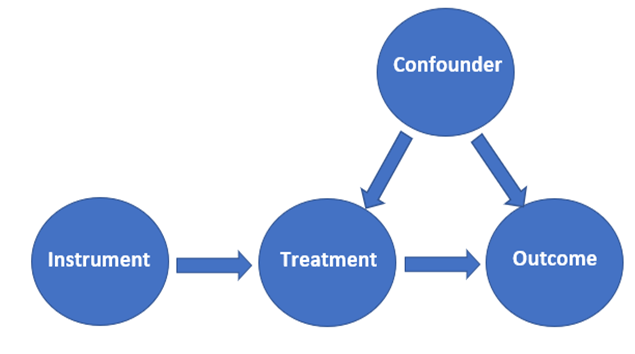
\includegraphics[scale=0.3]{notebooks/STATS/img/causal_inference_diagram.png}
    \caption{Casual Inference - DAG Diagram}
\end{figure}

Para resolver este problema, es necesario tomar algunos supuestos: 
\begin{enumerate}
    \item \textbf{Causal Markov Condition}: La influencia de las variables y el outcome puede ser representado a través de un \textbf{Grafo Acíclico Dirigido (DAG)} en el que se asume la \textbf{condición de Markov}, es decir si $Y \rightarrow S \rightarrow C$, podemos asumir que $C \indep Y | S$
    \item \textbf{SUTVA}: (Stable Unit Treatment Value Assumption) El grupo de control y tratamiento \textbf{no tiene influencia el uno con el otro}. 
    \item \textbf{Ignorability}: Se excluye el ruido proveniente de cualquier otra fuente. 
\end{enumerate}

Consideremos el siguiente ejemplo en el que buscamos determinar si el efecto de un tratamiento tiene un impacto en una variable target. 

\begin{figure}[H]
    \center
    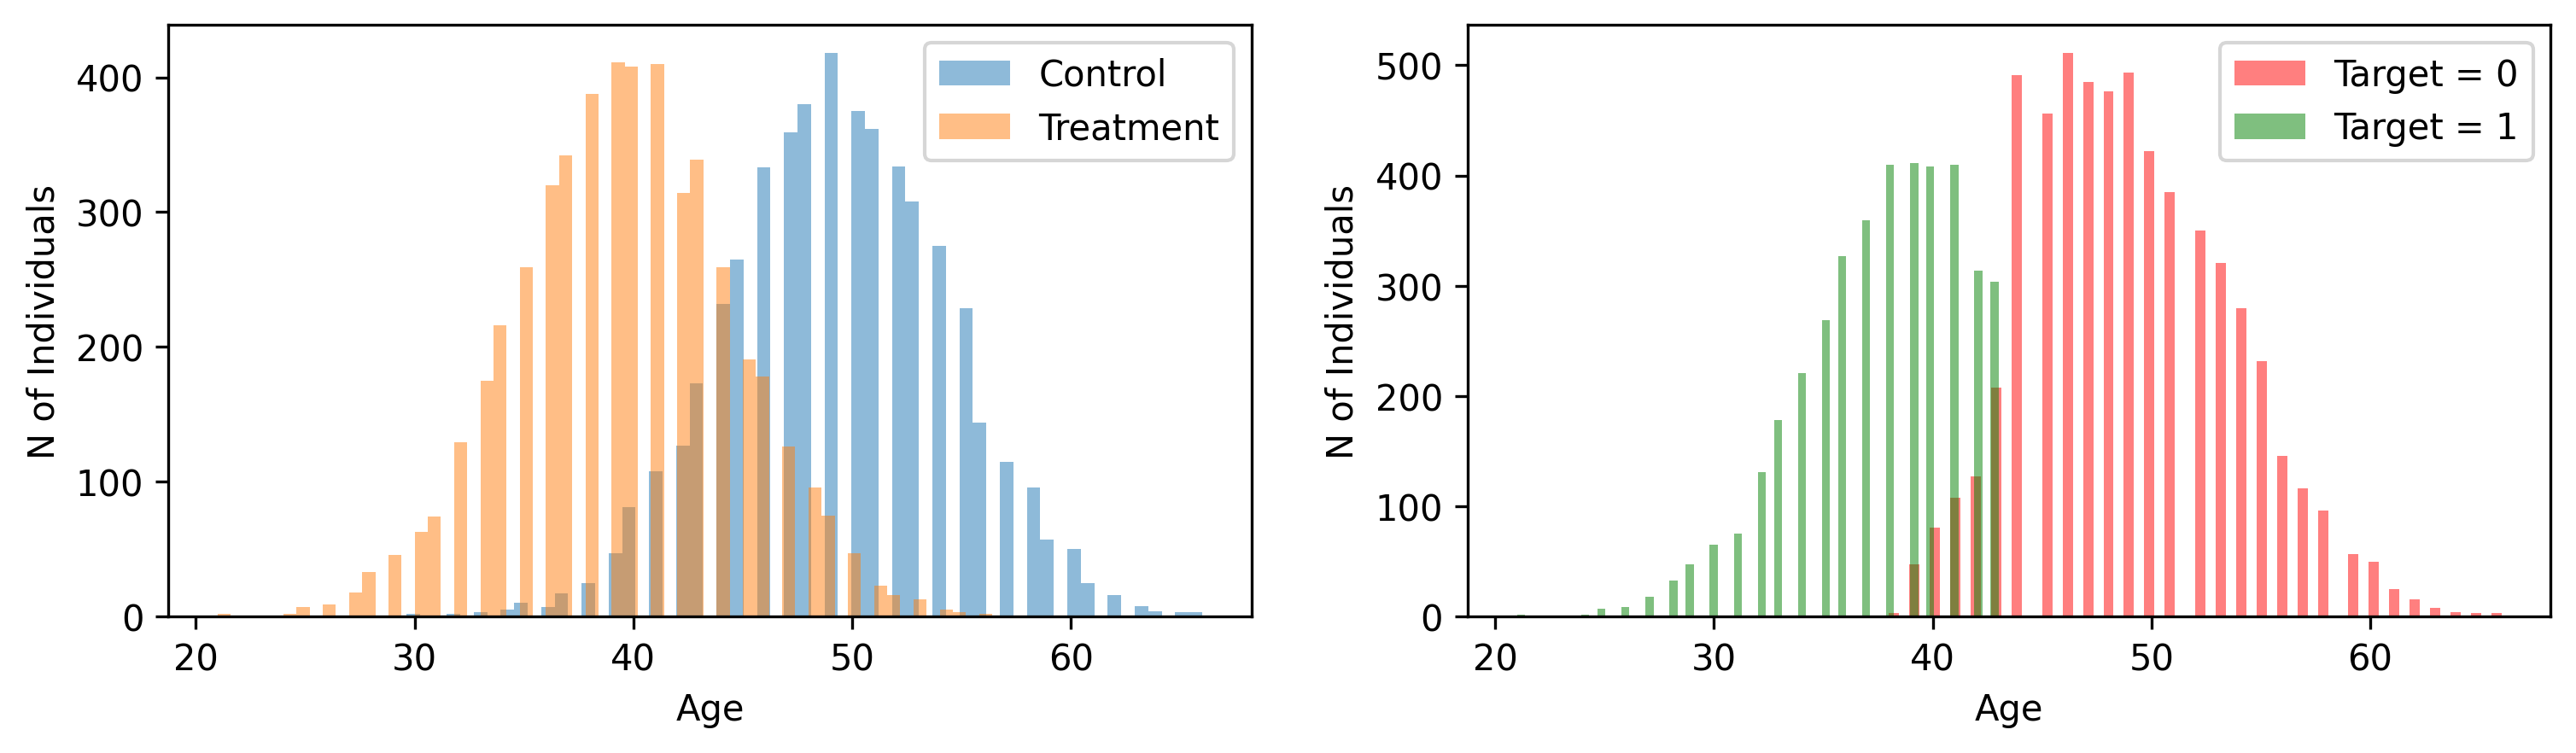
\includegraphics[scale=0.5]{notebooks/STATS/img/causal_inference_age_distribution.png}
    \caption{Casual Inference - Distribution Example}
\end{figure}

Vemos que existe un \textit{selection bias} pues el grupo de tratamiento y control tienen distribuciones de edad distintas. Existen múltiples enfoques para resolver este problema. 

\subsection{Matching Imputation}

Es posible utilizar un algoritmo de \textit{Matching} como \textit{NearestNeighbors} para imputar el posible outcome que hubiese tenido un individuo al recibir o no el tratamiento. En nuestro ejemplo, para cada edad de los individuos del grupo de control, buscaríamos al sujeto con la edad más cercana en el grupo de tratamiento e imputaríamos su respuesta al tratamiento y viceversa. 

La efectividad del tratamiento se puede medir a través del promedio de los outcome cuando reciben y cuando no reciben el tratamiento. 

\subsection{Meta Learners}

Este enfoque plantea utilizar algoritmos de \textit{Machine Learning} para determinar el efecto del tratamiento en el outcome del experimento. Sea $y_i$ el target, $w$ si recibió el tratamiento y $X_i$ el conjunto de variables del modelo, definimos ITE (\textit{Individual Treatment Effect}) según 
$$
\text{ITE} = \left [ p(y_i = 1 | w_i = 1, X_i) - p(y_i = 1 | w_i = 0, X_i) \right ]
$$

\begin{itemize}
    \item \textbf{S - Model} Este algoritmo es el más simple de todos pues agrega la variable \textit{treatment} como input de un único modelo. El valor de ITE es calculado para cada individuo variando el valor del tratamiento. 
    \item \textbf{T - Model} Este algoritmo entrena 2 clasificadores, uno encargado del grupo de control y otro para el grupo de tratamiento. El valor de ITE es calculado como la resta del output de ambos modelos. 

    Hay que tener en consideración que este modelo requiere una \textbf{calibración} para asegurar que el output de los modelos sean probabilidades.
    \item \textbf{X - Model}: SOON 
\end{itemize}


\begin{figure}[H]
    \center
    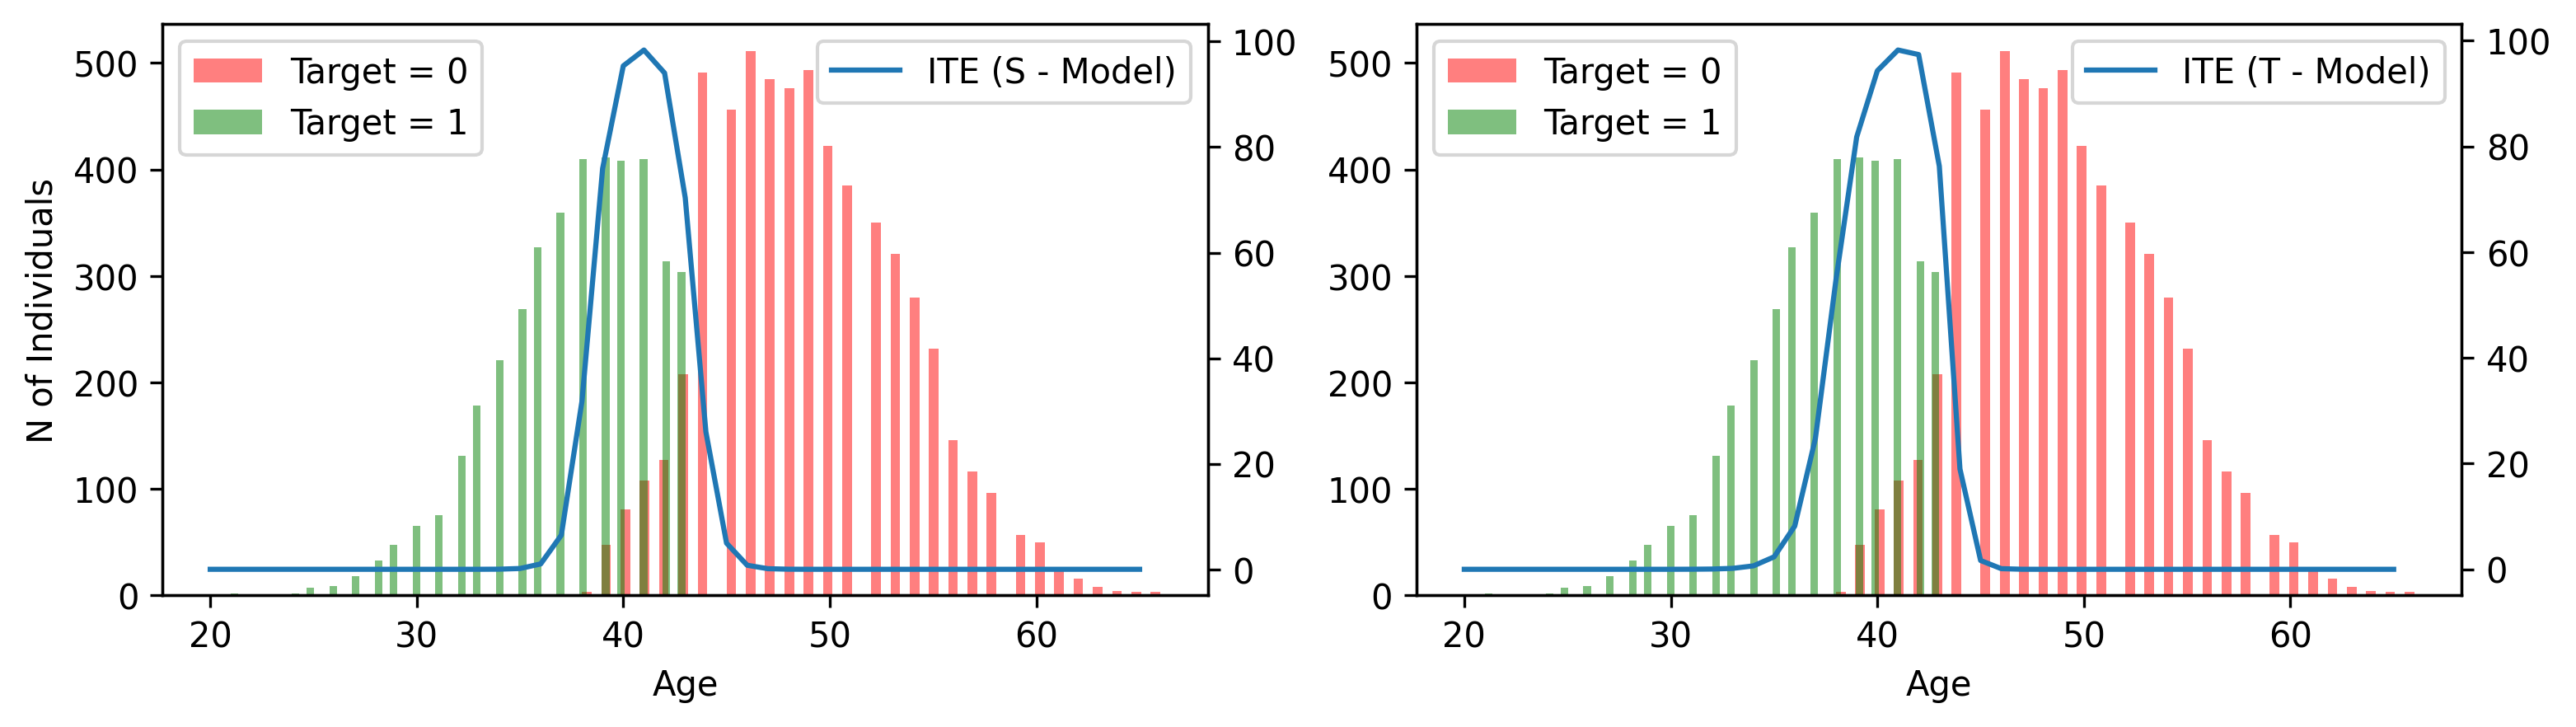
\includegraphics[scale=0.5]{notebooks/STATS/img/causal_inference_meta_learners.png}
    \caption{Meta Learners}
\end{figure}

Vemos así que el impacto del tratamiento aislando el efecto de la edad, ocurre según ITE entre los 35 y 45 años. 





